% File System (DONE)
\section{File system}
% ----------
\subsection{Systèmes de fichiers}
Pour les systèmes embarqués, il existe deux catégories de systèmes de fichiers :
\begin{enumerate}
    \item Volatiles (RAM)
    \item Persitants (Flash NOR et de plus en plus NAND)
\end{enumerate}
Deux technologies principales sont disponible sur les Flash :
\begin{itemize}
    \item MTD (Memory Technology Device)
    \item MMC/SD-Card (Multi-Media-Card/Secure Digital Card)
\end{itemize}

\begin{figure}[H]
    \centering
    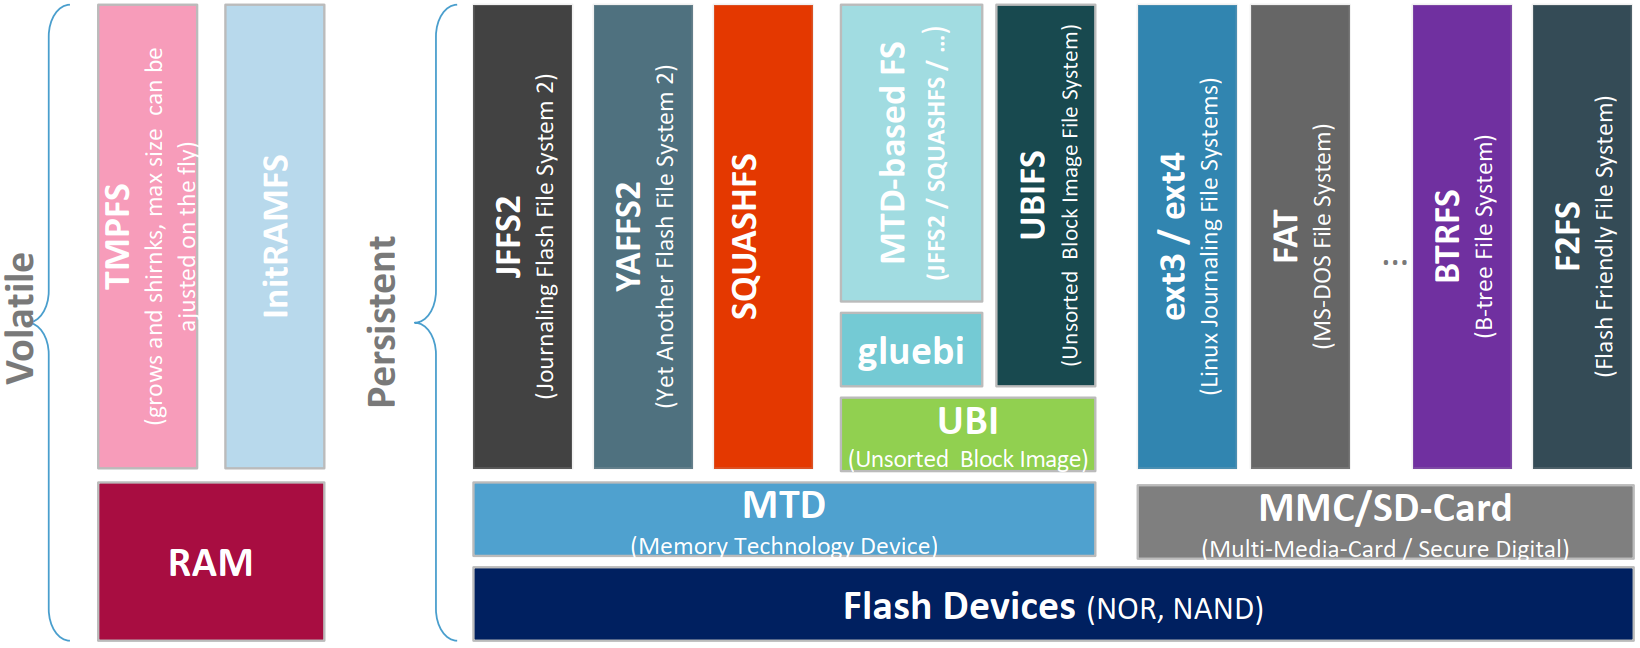
\includegraphics[width=\linewidth]{fileSystemType.png}
\end{figure}
% ----------
\subsubsection{Choix d'un FS}
\begin{figure}[H]
    \centering
    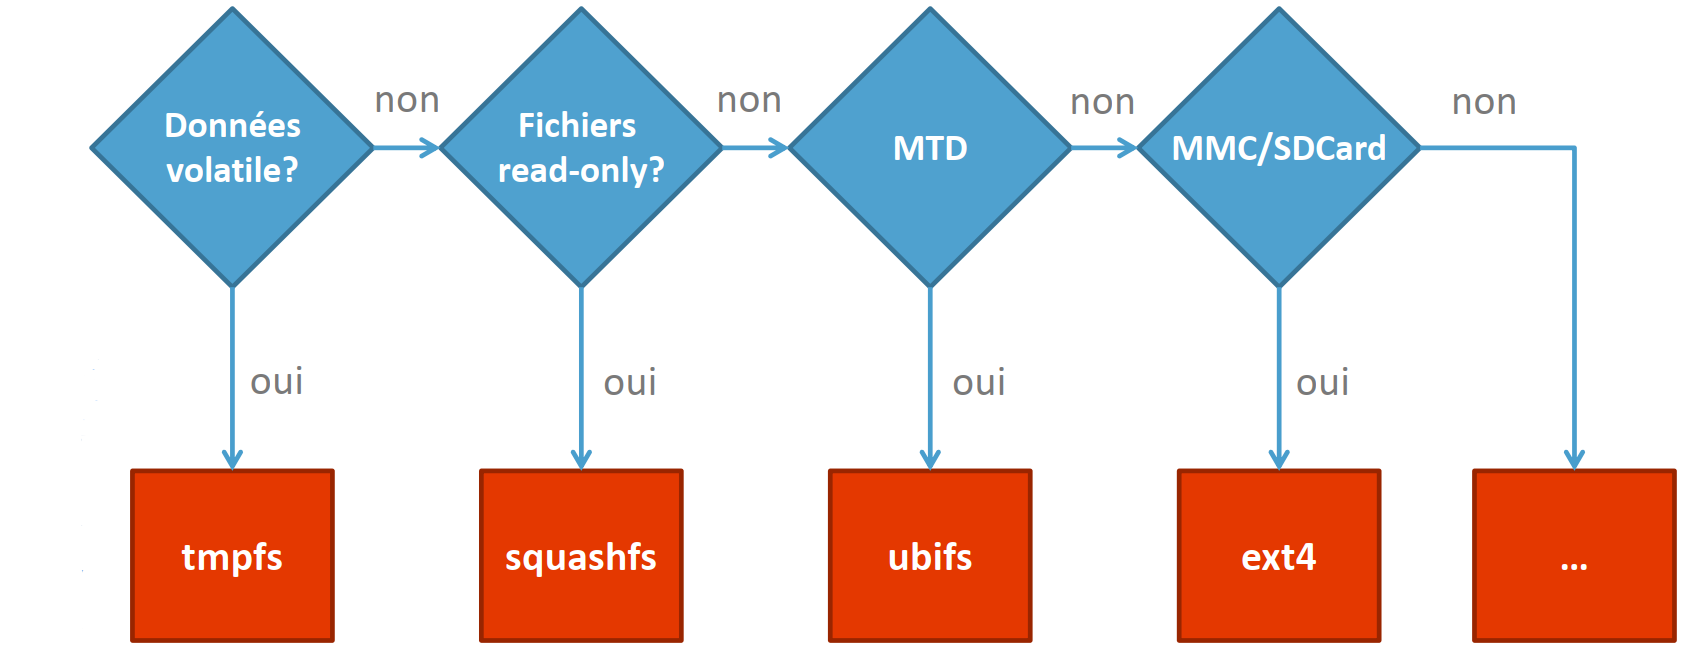
\includegraphics[width=\linewidth]{fileSystemChoice.png}
\end{figure}
% ----------
\subsubsection{MMC technologies}
MMC/eMMC/SD Card composés de 3 éléments :
\begin{itemize}
    \item MMC interface: Gère la communication avec l'hôte
    \item FTL (Flash translation layer)
    \item Zone de stockage (table de NAND)
\end{itemize}
% ----------
\paragraph{FTL}
Petit contrôleur qui fait tourner un firmware qui transforme l'adresse secteur logique en adresse NAND.
% ----------
\subsection{Architecture des FS}
% -----
\subsubsection{Journalisation}
Qui garde une trace de chaque modification dans un journal.

Permet la restauration de fichiers corrompus comme les fichiers sont d'abord écrite dans le journal avant d'être écrite sur le disque.
% -----
\subsubsection{B-Tree et CoW (Copy-on-Write)}
Architecture de stockage en arbre. Gère efficacement des grandes quantités de données en utilisant des nœuds qui contiennent plusieurs clés et valeurs, plutôt que des nœuds individuels.

La stratégie de CoW consiste à ne pas copier immédiatement les données lorsqu'une modification est apportée, mais copie que si cela s'avère nécessaire.
% -----
\subsubsection{Log FS}
Utilisation du support de stockage comme tampon circulaire $\Rightarrow$ les nouveaux blocs sont toujours écrits jusqu'à la fin.

\begin{figure}[H]
    \centering
    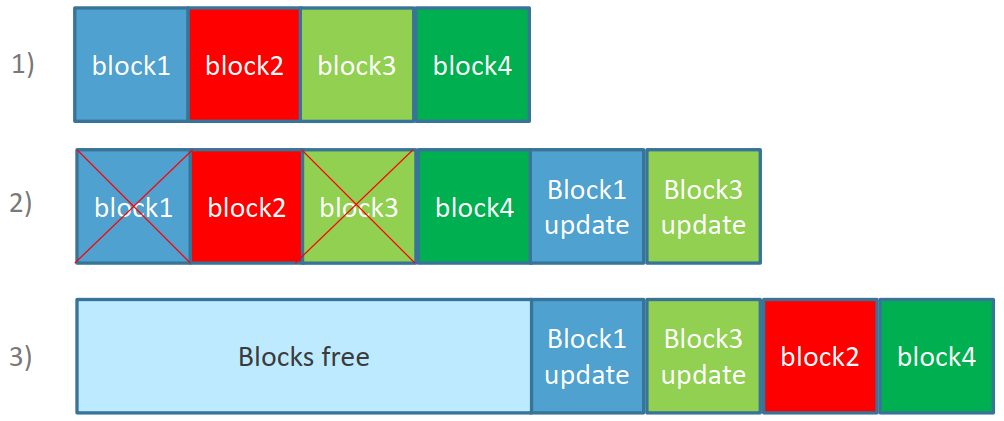
\includegraphics[width=0.8\columnwidth]{log_fs.png}
    \label{fig:log_fs}
\end{figure}
\begin{enumerate}
    \item Etat initial
    \item Modification des blocs 1 et 3
    \item Copie des blocs 2 et 4 dans une nouvelle zone avec les blocs 1 et 3 modifiés.
\end{enumerate}
% ----------
\subsection{Systèmes de fichiers alternatifs}
\paragraph{BTRFS} : système récent (2007, stable 2014), système B-Tree, potentiellement meilleur que ext4 (selon développeur principal de ext4).
\paragraph{F2FS (Flash-Friendly File System)} : log FS, opérations atomiques (exécuté sans interruption), défragmentation, support du TRIM (informe qu'un bloc de données n'est plus utilisé et peut être supprimé).
\paragraph{XFS} : journalisé, support de très gros FS, designé pour être extensible, il ne semble cependant pas bien gérer les pertes de puissance (état de veille).
\paragraph{NILFS2} : Log FS et B-Tree, Userspace garbage collector.
\paragraph{ZFS} : B-Tree, support de FS volumineux, pas très adapté à l'embarqué (utilise RAM).
% ----------
\subsection{Ext2-3-4}
\paragraph{Ext2} : non journalisé, utilise le block mapping pour réduire la fragmentation
\paragraph{Ext3} : (2001), journalisé, prévient la perte de donnée même en cas de d'extinction brutale du système contrairement à Ext2, rétro-compatible vec ext2.
\paragraph{Ext4} : (2008), actuellement meilleur FS pour l'embarqué utilisant MMC, rétro-compatible avec ext3 et ext4, supporte système de fichiers volumineux, utilisation des extents.

Les extents permettent de regrouper plusieurs blocs consécutifs de données en un seul objet appelé "extent", ce qui permet d'optimiser les performances d'écriture et de lecture. les extents permettent également de réduire le nombre de métadonnées nécessaires pour stocker les informations sur l'emplacement des données d'un fichier, ce qui permet d'économiser de l'espace disque et d'améliorer les performances.
% ----------
\subsection{SquashFS}
Linux FS compressé, lecture seule.

Destiné à une utilisation générale en lecture seule, à une utilisation archivistique et dans les systèmes embarqués avec de petits processeurs où de faibles charges sont nécessaires.
% ----------
\subsection{Tmpfs}
Garde tous les fichiers en mémoire virtuelle. Tout dans tmpfs est temporaire. Si une instance tmpfs est démontée, tout ce qui y est stocké est perdu.
Tmpfs est un système de fichier en mémoire qui permet de stocker des fichiers temporaires qui ont besoin d'un accès rapide aux données, d'utiliser l'espace libre de la mémoire vive, d'être sécurisé pour les données sensibles et d'être flexible pour stocker différents types de fichiers temporaires.
\subsubsection{Devtmpfs}
Devtmpfs est un système de fichiers qui remplit automatiquement les fichiers de nœuds (/dev) connus du noyau.
% ----------
\subsection{LUKS (Linux Unified Key Setup)}
Système de chiffrement de disque utilisé pour chiffrer les partitions de disque sur les systèmes Linux. Protège les données sur le disque en utilisant une clé de chiffrement qui est utilisée pour chiffrer les données sur le disque. Lorsqu'un utilisateur veut accéder à des données chiffrées sur le disque, il doit d'abord entrer la clé de chiffrement pour déchiffrer les données.
% ----------
\subsection{Conclusion}
Performances:
\begin{itemize}
    \item EXT4: meilleure solution pour les systèmes embarqués utilisant MMC
    \item F2FS et NILFS2 hautes performances en écriture
\end{itemize}
Features:
\begin{itemize}
    \item BTRFS FS de prochaine génération
    \item NILFS2 Fournit des fonctionnalités plus simples mais similaires
\end{itemize}
Scalability:
\begin{itemize}
    \item EXT4 n'évolue clairement pas aussi bien que BTRFS et F2FS
\end{itemize}
\begin{figure}[H]
    \centering
    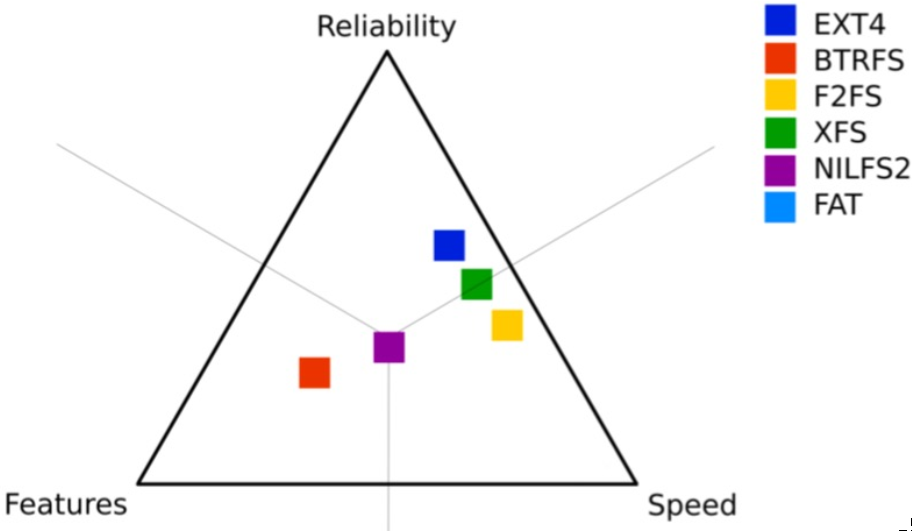
\includegraphics[width=0.6\columnwidth]{fsComp.png}
    \label{fig:fsComp}
\end{figure}
